% ISRO-BAH-26 -- Technical report: architecture and mathematics
% Build: pdflatex ISRO-BAH-26_Technical_Report.tex   (run twice for the table of contents)
\documentclass[11pt,a4paper]{article}

\usepackage[margin=2.3cm]{geometry}
\usepackage[T1]{fontenc}
\usepackage[utf8]{inputenc}
\usepackage{lmodern}
\usepackage{amsmath,amssymb}
\usepackage{booktabs}
\usepackage{tabularx}
\usepackage{xcolor}
\usepackage{enumitem}
\usepackage{graphicx}
\usepackage{float}
\usepackage{tikz}
\usetikzlibrary{arrows.meta,positioning,fit,backgrounds}
\usepackage[colorlinks=true,linkcolor=blue!50!black,urlcolor=blue!50!black]{hyperref}

\definecolor{accent}{HTML}{3C78B4}
\newcommand{\code}[1]{\texttt{#1}}
\newcommand{\Pice}{P(\text{ice})}
\DeclareMathOperator{\logit}{logit}
\DeclareMathOperator{\MAD}{MAD}
\DeclareMathOperator{\med}{med}
\setlist{itemsep=2pt,topsep=4pt}
\setlength{\emergencystretch}{3em}
\sloppy

\title{\textbf{ISRO-BAH-26}\\[4pt]\large Subsurface ice mapping and rover traverse planning
at the lunar south pole with Chandrayaan-2 DFSAR\\[2pt]
\normalsize Architecture, mathematics and results}
\author{Team Nakshatra: Avinash Chandra Gupta, Subodh Bansal, Esha Jain\\
\small \url{https://github.com/Avinashistoocool/ISRO-BAH-26}}
\date{Version 1.0.0 \quad October 2026}

\begin{document}
\maketitle

\begin{abstract}
This report documents the code submitted by team Nakshatra for the ISRO Bharatiya Antariksh
Hackathon 2026 problem on detecting and characterising subsurface water ice in lunar south polar
regions for landing-site and rover-traverse planning. The study area is a
$60\times60$\,km window around Faustini crater on the LOLA 20\,m south-polar DEM. Six public
evidence layers (LOLA PSR map, LOLA solar visibility, Diviner maximum temperature and
depth-to-ice-stability, Mini-RF S-band CPR, LAMP Lyman-$\alpha$ ratio) and the Chandrayaan-2 DFSAR
L-band Level-3C polar mosaic are resampled onto the DEM grid. Ice probability is computed by
naive-Bayes evidence fusion in log-odds space, gated by a thermal-stability term, with
Monte-Carlo propagation of weight uncertainty. A dual-frequency (L/S) inversion turns the
roughness-corrected CPR excess in each band into a depth to the top of the ice, and an
enrichment test decides whether that depth map is trusted. An expected ice volume in the top
5\,m is integrated for three assumed ice volume fractions. A separate module builds a
slope-based traversability cost map and plans a rover path with 8-connected A*. All formulas
below are taken from the code, with the constants it actually uses, and the results section
reports only numbers that are committed in the repository.
\end{abstract}

\tableofcontents
\newpage

%====================================================================
\section{Motivation}
%====================================================================

Craters inside the permanently shadowed regions (PSRs) near the lunar south pole never see direct
sunlight. Their floors stay below about 110\,K, cold enough for water ice to survive over
geological time. Some of these craters are \emph{doubly shadowed}: they are also hidden from
the sunlit walls that would otherwise heat them by scattered and thermal radiation. Knowing
where ice is, how deep it lies and whether a rover can reach it is a prerequisite for any future
Indian polar mission.

The hackathon problem statement asks for five things: a subsurface ice map from Chandrayaan-2
dual-frequency SAR (DFSAR), a fused terrain and ice-probability map, an ice volume estimate for
the top few metres of regolith, a safe landing site, and an energy-aware rover traverse. The
repository implements the first three as a calibrated, uncertainty-aware pipeline, and the last
two as a working A* planner on a slope cost map plus a landing-site prototype. Reinforcement
learning, the orbiter/relay communication simulation and OHRC hazard mapping are described in
the README and the pitch deck but are not yet in the code (Section~\ref{sec:limits}).

\subsection{Why radar alone is not enough}
The classic radar signature of ice is a high circular polarisation ratio (CPR), caused by
coherent backscatter from low-loss ice. Rough, blocky terrain produces the same signature, which
is why fresh crater rims and ejecta show CPR above one without any ice. An earlier heuristic
version of this project used a fixed \(\mathrm{CPR}>1\) threshold and fixed weights. According to
the README it marked about 3600\,km$^2$ as likely ice, and 61\,\% of that lay in terrain with
\(T_{\max}>150\)\,K, where ice cannot survive. The current model was built to fix that: radar is
corrected for roughness using ice-free terrain as a reference, and every probability is
multiplied by a physical thermal-stability term.

%====================================================================
\section{Architecture}
%====================================================================

The repository is a set of flat Python modules. Two independent chains share the same DEM
source and projection (Figure~\ref{fig:pipeline}).

\begin{figure}[H]
\centering
\resizebox{\linewidth}{!}{%
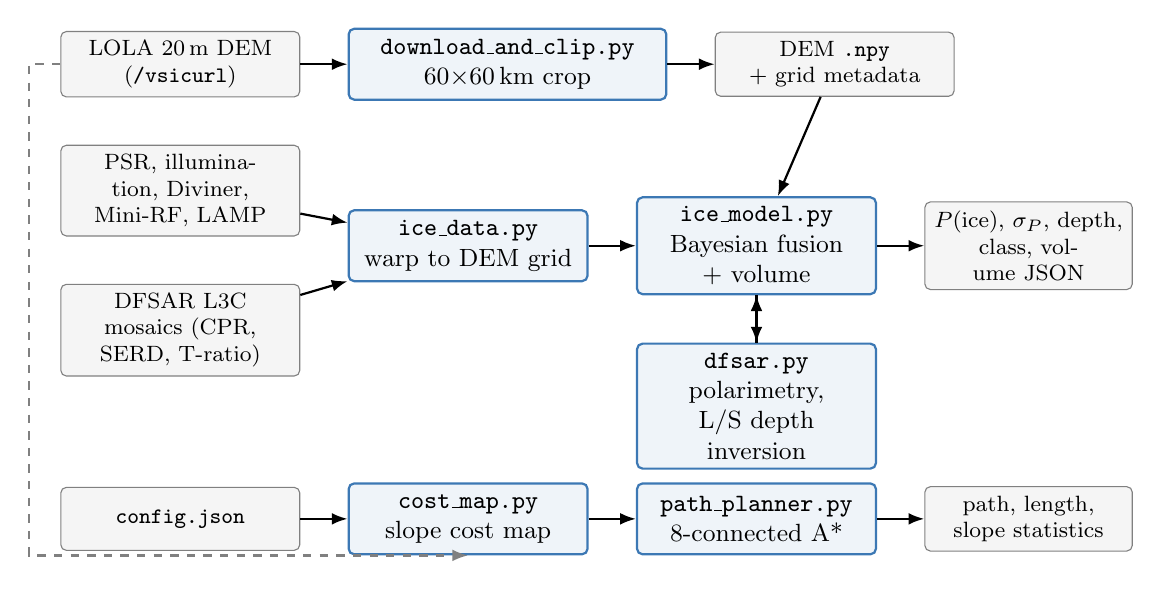
\begin{tikzpicture}[
  node distance=6mm and 6mm,
  box/.style={draw=accent,thick,rounded corners=2pt,fill=accent!8,align=center,
              font=\small,minimum height=9mm,text width=28mm},
  data/.style={draw=gray,rounded corners=2pt,fill=gray!8,align=center,font=\footnotesize,
               text width=28mm,minimum height=8mm},
  arr/.style={-{Latex[length=2mm]},thick}]
  \node[data] (lola) {LOLA 20\,m DEM\\(\code{/vsicurl})};
  \node[box,right=of lola,text width=38mm] (clip) {\code{download\_and\_clip.py}\\60$\times$60\,km crop};
  \node[data,right=of clip] (npy) {DEM \code{.npy}\\+ grid metadata};
  \node[data,below=of lola] (pub) {PSR, illumination, Diviner, Mini-RF, LAMP};
  \node[data,below=of pub] (dfs) {DFSAR L3C mosaics (CPR, SERD, T-ratio)};
  \node[box,right=of pub,yshift=-7mm] (data) {\code{ice\_data.py}\\warp to DEM grid};
  \node[box,right=of data] (model) {\code{ice\_model.py}\\Bayesian fusion\\+ volume};
  \node[box,below=of model] (dual) {\code{dfsar.py}\\polarimetry,\\L/S depth inversion};
  \node[data,right=of model,text width=24mm] (out) {$\Pice$, $\sigma_P$, depth,\\class, volume JSON};
  \node[data,below=14mm of dfs] (cfg) {\code{config.json}};
  \node[box,right=of cfg] (cost) {\code{cost\_map.py}\\slope cost map};
  \node[box,right=of cost] (plan) {\code{path\_planner.py}\\8-connected A*};
  \node[data,right=of plan,text width=24mm] (path) {path, length,\\slope statistics};
  \draw[arr] (lola) -- (clip);
  \draw[arr] (clip) -- (npy);
  \draw[arr] (npy) -- (model);
  \draw[arr] (pub) -- (data);
  \draw[arr] (dfs) -- (data);
  \draw[arr] (data) -- (model);
  \draw[arr] (model) -- (dual);
  \draw[arr] (dual) -- (model);
  \draw[arr] (model) -- (out);
  \draw[arr] (cfg) -- (cost);
  \draw[arr] (cost) -- (plan);
  \draw[arr] (plan) -- (path);
  \draw[arr,dashed,gray] (lola.west) -- ++(-4mm,0) |- (cost.south);
\end{tikzpicture}}
\caption{Processing chains. Top: ice-distribution model. Bottom: traverse planner, which
streams its own DEM window (dashed) around the centre given in \code{config.json}.}
\label{fig:pipeline}
\end{figure}

\begin{center}
\begin{tabularx}{\linewidth}{@{}lX@{}}
\toprule
Module & Role \\
\midrule
\code{download\_and\_clip.py} & Streams a square window of the LOLA 80\textdegree S 20\,m DEM and
writes \code{lunar\_south\_pole\_full.npy} plus \code{\_meta.json} (origin, pixel size, WKT). \\
\code{ice\_data.py} & Downloads only the window of each evidence layer that covers the crop and
resamples it onto the DEM grid; caches to \code{data/processed/*.npy}. \\
\code{dfsar.py} & Compact- and full-pol CPR/DOP, roughness-corrected CPR excess, L/S detection
classes, depth inversion with Monte-Carlo noise, enrichment test. \\
\code{ice\_model.py} & Terrain roughness, evidence layers, log-odds fusion, thermal gate,
volume integration, GeoTIFF/PNG/JSON export. \\
\code{cost\_map.py} & Config loading, lat/lon to pixel, DEM clip, slope, cost map, snapping of
start/goal to passable cells. \\
\code{path\_planner.py} & A* search, path length and slope statistics, plotting. \\
\code{landing\_site.py} & Prototype site-suitability index (slope + illumination). \\
\code{all\_maps.py}, \code{scripts/} & Visualisation and slope/roughness diagnostics. \\
\code{tests/test\_dfsar.py} & Synthetic tests of the polarimetry and the depth inversion. \\
\bottomrule
\end{tabularx}
\end{center}

%====================================================================
\section{Data and coordinate system}
%====================================================================

\subsection{Sources}
All layers are read through GDAL \code{/vsicurl}, so only the bytes covering the crop are
transferred.

\begin{center}
\begin{tabularx}{\linewidth}{@{}lXl@{}}
\toprule
Layer & Product & Resampling \\
\midrule
DEM & LOLA \code{LDEM\_80S\_20MPP\_ADJ}, 20\,m & -- \\
PSR & LOLA \code{LPSR\_80S\_20MPP\_ADJ}, 20\,m (Barker et al.) & nearest \\
Illumination & LOLA average solar visibility 85--90\textdegree S, 60\,m (Mazarico et al.\ 2011) & bilinear \\
$T_{\max}$ & Diviner south-polar summer maximum temperature (Williams et al.\ 2019) & bilinear \\
Ice depth & Diviner depth to ice stability, 240\,m (Schorghofer \& Williams 2020) & bilinear \\
CPR$_S$ & LRO Mini-RF S-band (12.6\,cm) CPR mosaic, 118\,m & average \\
LAMP & LRO LAMP Lyman-$\alpha$ off/on-band albedo ratio, 240\,m (Gladstone 2012) & bilinear \\
DFSAR & Chandrayaan-2 DFSAR L-band Level-3C polar mosaic, 25\,m (CPR, SERD, T-ratio) & average \\
\bottomrule
\end{tabularx}
\end{center}

DFSAR requires an ISSDC PRADAN account. The loader looks for the Level-3C files under
\code{data/raw/dfsar/data/derived/} (south-polar east and west tiles) and for optional flat files
\code{dfsar\_cpr\_S.tif}, \code{dfsar\_dop\_L.tif}, \code{dfsar\_dop\_S.tif}. Only L-band CPR,
SERD and T-ratio were available for the committed run, so the S-band of the dual-frequency
inversion is Mini-RF (both are 12.6\,cm). The illumination and T-ratio layers are fetched but not
yet used by the model.

\subsection{Projection and grid}
Every source uses the IAU 30135 south polar stereographic projection on a sphere of radius
$R=1\,737\,400$\,m (polar stereographic variant B, standard parallel $-90^\circ$, longitude
of origin $0^\circ$). For a point at latitude $\varphi$ and longitude $\lambda$ the projected
coordinates are
\begin{equation}
  \rho = 2R\tan\!\left(\frac{\pi}{4}+\frac{\varphi}{2}\right),\qquad
  x = \rho\sin\lambda,\qquad y = \rho\cos\lambda ,
\end{equation}
which \code{pyproj} evaluates with the sphere radius read from the raster's own CRS rather than
hard-coded. The crop is centred on $(-87.85^\circ, 82.0^\circ)$ with half-width 30\,km, giving a
$3000\times3000$ grid of $p=20$\,m pixels with top-left corner $(x_0,y_0)=(34\,560, 39\,080)$\,m.
Pixel indices follow from the affine transform
\begin{equation}
  c = \operatorname{round}\!\left(\frac{x-x_0}{p}\right),\qquad
  r = \operatorname{round}\!\left(\frac{y_0-y}{p}\right),
\end{equation}
and the inverse $x=x_0+cp$, $y=y_0-rp$ is used to convert a path back to latitude and longitude.

\subsection{Resampling}
\code{warp\_to\_grid} reads the source window that covers the target bounds plus a pad of four
source pixels, replaces nodata (and values below $-10^{30}$) with NaN, applies the band scale and
offset, and reprojects with the resampling method in the table above. Averaging is used for
radar so that one 20\,m output cell represents the mean backscatter of the coarser source cell.

%====================================================================
\section{Terrain derivatives}
%====================================================================

\subsection{Slope}
With central differences $g_x=\partial z/\partial x$, $g_y=\partial z/\partial y$ computed by
\code{numpy.gradient} at spacing $p$,
\begin{equation}
  s = \frac{180}{\pi}\arctan\sqrt{g_x^2+g_y^2}\quad[\text{deg}].
\end{equation}
This is the same formula in \code{cost\_map.py}, \code{ice\_model.py}, \code{landing\_site.py}
and \code{scripts/diagnostic.py}.

\subsection{Radar-scale roughness}
Radar responds to roughness at the scale of its footprint, not of the DEM pixel. The model
therefore uses the RMS slope inside a boxcar window matched to the Mini-RF resolution
($L_r=120$\,m):
\begin{equation}
  \rho_{\mathrm{DEM}} = \sqrt{\big\langle s^2\big\rangle_{k\times k}},\qquad
  k=\operatorname{round}(L_r/p)=6 .
\end{equation}
When the DFSAR SERD layer (surface-roughness descriptor, high for smooth surfaces) is
available it replaces this covariate, because on this crop SERD explains about 75\,\% of the
L-band CPR variance against about 0.5\,\% for DEM roughness:
\begin{equation}
  \rho_{\mathrm{radar}} = -\,\overline{\mathrm{SERD}}_{k\times k},
\end{equation}
where $\overline{\,\cdot\,}$ is a NaN-aware boxcar mean that returns NaN if less than half of the
window is valid. The visualisation scripts use a different, purely illustrative roughness,
$|z-G_{\sigma=2}*z|$ (absolute residual from a Gaussian-smoothed DEM).

%====================================================================
\section{Radar polarimetry (\code{dfsar.py})}
%====================================================================

\subsection{Compact (hybrid) polarimetry}
DFSAR's hybrid mode transmits a circular wave and receives linear H and V. With multilooking
$\langle\cdot\rangle$ (a boxcar of $5\times1$ looks in azimuth and range by default) the
received Stokes vector is (Raney 2007)
\begin{align}
  S_1 &= \langle |E_H|^2+|E_V|^2\rangle, & S_2 &= \langle |E_H|^2-|E_V|^2\rangle,\\
  S_3 &= 2\,\mathrm{Re}\langle E_H E_V^*\rangle, & S_4 &= -2\,\mathrm{Im}\langle E_H E_V^*\rangle,
\end{align}
and
\begin{equation}
  \mathrm{CPR} = \frac{S_1-S_4}{S_1+S_4},\qquad
  \mathrm{DOP} = \frac{\sqrt{S_2^2+S_3^2+S_4^2}}{S_1}\in[0,1].
\end{equation}
For left-circular transmit the sign of $S_4$ flips. Denominators are floored at $10^{-12}$.

\subsection{Full polarimetry}
For a linear-basis scattering matrix with reciprocity $S_{HV}=S_{VH}$, the same-sense and
opposite-sense circular returns are
\begin{equation}
  S_{\mathrm{SC}} = \tfrac12\,(S_{HH}-S_{VV}+2jS_{HV}),\qquad
  S_{\mathrm{OC}} = \tfrac{j}{2}\,(S_{HH}+S_{VV}),\qquad
  \mathrm{CPR} = \frac{\langle|S_{\mathrm{SC}}|^2\rangle}{\langle|S_{\mathrm{OC}}|^2\rangle}.
\end{equation}
The common factor $\tfrac14$ cancels, so the code multilooks $|S_{HH}-S_{VV}+2jS_{HV}|^2$ and
$|S_{HH}+S_{VV}|^2$ directly. A flat surface or sphere ($S_{HH}=S_{VV}$, $S_{HV}=0$) gives
$\mathrm{CPR}\to0$; a dihedral ($S_{HH}=-S_{VV}$) gives $\mathrm{CPR}\to\infty$. Both limits are
unit-tested.

\subsection{Multilook factor}
To obtain approximately square ground pixels (ISRO MIDAS convention) the number of azimuth looks
is
\begin{equation}
  n_{\mathrm{az}} = \max\!\left(1,\operatorname{round}\frac{\Delta_{\mathrm{px}}}
  {\Delta_{\mathrm{line}}\sin\theta_i}\right),
\end{equation}
with one look in range, where $\theta_i$ is the incidence angle.

%====================================================================
\section{Ice-probability model (\code{ice\_model.py})}
%====================================================================

\subsection{Robust standardisation}
All evidence is converted to robust $z$-scores using the median and the scaled median absolute
deviation of a reference set $\mathcal{R}$:
\begin{equation}
  z(x) = \frac{x-\med_{\mathcal{R}}(x)}{1.4826\,\MAD_{\mathcal{R}}(x)+10^{-9}},
\end{equation}
with NaN mapped to $0$ (no evidence). The factor 1.4826 makes the MAD a consistent estimator of
the standard deviation for Gaussian data.

\subsection{Thermal stability gate}
Surface ice is stable where the annual maximum temperature is below $T_s=110$\,K. The
transition is softened with width $\tau=5$\,K. Diviner's depth-to-ice-stability $z_{\mathrm{ice}}$
adds a capped subsurface term:
\begin{equation}
  P_{\mathrm{stab}} = \max\!\left(\sigma\!\left(\frac{T_s-T_{\max}}{\tau}\right),\;
  0.6\,e^{-z_{\mathrm{ice}}/0.05\,\mathrm{m}}\right),
  \qquad \sigma(u)=\frac1{1+e^{-u}},
\end{equation}
where the second term is zero if $z_{\mathrm{ice}}$ is undefined. The cap of $0.6$ is deliberate:
the stability depth is finite over most of the region, so a shallow stability depth raises the
chance of ice but never as strongly as a cold surface does.

\subsection{Roughness-corrected CPR anomaly}
Pixels with $T_{\max}>150$\,K cannot hold ice and therefore show what roughness alone does to
CPR. On these \emph{warm} pixels the code fits
\begin{equation}
  \ln\mathrm{CPR} = a + b\,\rho ,
\end{equation}
robustly: the warm pixels are split into 20 quantile bins of $\rho$, and an ordinary least-squares
line is fitted through the 20 (median $\rho$, median $\ln\mathrm{CPR}$) pairs. CPR is clipped at
$10^{-3}$ before the logarithm. The evidence is the standardised residual
\begin{equation}
  e_{\mathrm{cpr}} = z_{\mathrm{warm}}\!\big(\ln\mathrm{CPR}-(a+b\rho)\big),
\end{equation}
where the median and MAD are taken over warm pixels, so that ice-free terrain has $z\approx0$ by
construction. For Mini-RF the fit uses the DEM roughness. For DFSAR L-band CPR (first smoothed to
the 120\,m scale) it uses $\rho_{\mathrm{radar}}$, and the DFSAR term is only fused if the mean
anomaly of cold pixels ($T_{\max}<110$\,K) exceeds that of warm pixels:
\begin{equation}
  \Delta z = \overline{e}_{\mathrm{cold}}-\overline{e}_{\mathrm{warm}} > 0 .
\end{equation}

\subsection{LAMP frost evidence}
The LAMP off-band/on-band ratio $r$ rises above one where surface frost is present. Values
outside $0<r<10$ are discarded as artefacts, and
\begin{equation}
  e_{\mathrm{lamp}} = \operatorname{clip}\!\big(\langle z(\ln r)\rangle_{12\times12},\,-3,\,3\big),
\end{equation}
i.e.\ the $z$-score is smoothed over 12 pixels (240\,m, the LAMP resolution) and clipped.

\subsection{Log-odds fusion}
With the PSR mask $e_{\mathrm{psr}}\in\{0,1\}$ and an optional DFSAR DOP term
(low DOP indicates volume scattering, hence the minus sign), the log-odds are
\begin{equation}
  \ell = \ell_0 + w_{\mathrm{cpr}}e_{\mathrm{cpr}} + w_{\mathrm{lamp}}e_{\mathrm{lamp}}
       + w_{\mathrm{psr}}e_{\mathrm{psr}} + w_{\mathrm{dfsar}}e_{\mathrm{dfsar}}
       - w_{\mathrm{dop}}\,z(\mathrm{DOP}),
\end{equation}
and the probability is gated by thermal stability:
\begin{equation}
  \Pice = P_{\mathrm{stab}}\;\sigma(\ell).
\end{equation}
Only terms whose layers exist enter the sum. There are no ground-truth ice labels, so the weights
cannot be fitted. They are instead treated as uncertain: each of $N=64$ Monte-Carlo draws samples
$w_j\sim\max\!\big(0,\mathcal{N}(\mu_j,s_j^2)\big)$, and the output is the per-pixel mean and
standard deviation of $\Pice$ over the draws.

\begin{center}
\begin{tabular}{@{}lcc@{}}
\toprule
Term & $\mu_j$ & $s_j$ \\
\midrule
Prior $\ell_0$ & $-1.5$ & -- \\
Mini-RF CPR anomaly & 0.8 & 0.3 \\
LAMP & 0.5 & 0.25 \\
PSR & 1.5 & 0.5 \\
DFSAR CPR anomaly & 1.2 & 0.4 \\
DFSAR DOP (negative sign) & 0.8 & 0.3 \\
\bottomrule
\end{tabular}
\end{center}

The prior $\ell_0=-1.5$ corresponds to $\sigma(-1.5)\approx0.18$. A PSR pixel with no other
evidence and a cold surface therefore has $\Pice\approx\sigma(0)=0.5$.

%====================================================================
\section{Dual-frequency depth inversion (\code{dfsar.py})}
%====================================================================

\subsection{CPR excess and detection}
For each band $b\in\{L,S\}$ the CPR excess over the rough-terrain baseline is computed in
linear units, with the baseline fitted on warm pixels exactly as above:
\begin{equation}
  e_b = \mathrm{CPR}_b - \exp(a_b+b_b\rho_{\mathrm{radar}}),\qquad
  \sigma_b = 1.4826\,\MAD_{\mathrm{warm}}(e_b),\qquad z_b = e_b/\sigma_b .
\end{equation}
A band detects ice where $z_b>3$ and, if a DOP layer exists, $\mathrm{DOP}_b<0.13$ (the
volume-scattering threshold from the problem statement). Each pixel gets one class:

\begin{center}
\begin{tabular}{@{}cll@{}}
\toprule
Class & Condition & Meaning \\
\midrule
0 & neither band & no detection \\
1 & L and S & near-surface ice, within S-band reach \\
2 & L only & deep ice, below S-band reach \\
3 & S only & physically inconsistent (roughness or calibration) \\
\bottomrule
\end{tabular}
\end{center}

\subsection{Two-layer attenuation model}
Model the ice as a layer whose top is at depth $D$ under a dry regolith lag. Band $b$'s
sensitivity decays exponentially with e-folding depth $\delta_b$, and $k_b$ is its scattering
efficiency for an ice amount $A$:
\begin{equation}
  e_b = A\,k_b\,e^{-D/\delta_b}.
\end{equation}
The code uses $\delta_S=0.5$\,m and $\delta_L=1.5$\,m (sensing depth of roughly two e-folds:
about 1\,m for S and 3\,m for L). The ratio of the two bands cancels $A$:
\begin{equation}
  R=\frac{e_L}{e_S}=k\,\exp\!\left[D\left(\frac1{\delta_S}-\frac1{\delta_L}\right)\right],
  \qquad k=\frac{k_L}{k_S},
\end{equation}
so
\begin{equation}
  D = \frac{\ln e_L-\ln e_S-\ln k}{1/\delta_S-1/\delta_L}
    = \frac{\ln(R/k)}{1.333\,\mathrm{m}^{-1}},
  \qquad D\in[0,\,D_{\max}=5\,\mathrm{m}].
\end{equation}
If $e_S\le0$ (S-band sees nothing) the depth is set to $D_{\max}$.

\subsection{Calibrating $k$}
Where $T_{\max}<100$\,K surface ice is stable and $D\approx0$, so $R\approx k$. The calibration
uses pixels that are that cold and detected in both bands ($e_b>3\sigma_b$):
\begin{equation}
  \ln k = \med\big(\ln e_L-\ln e_S\big),
\end{equation}
and requires at least 200 such pixels; otherwise $\ln k=0$ and the result is flagged as
uncalibrated. The synthetic test generates $k=1.3$ and checks the recovered value to $\pm0.1$.

\subsection{Noise propagation}
Depth is estimated by Monte Carlo with 32 samples:
$\tilde e_b = e_b+\mathcal{N}(0,\sigma_b^2)$. Samples with $\tilde e_L\le0$ are discarded, and
the per-pixel mean and standard deviation of $D(\tilde e_L,\tilde e_S)$ over the remaining
samples are returned. Depth is NaN where L-band does not detect ice, for class~3, and where any
input is missing.

\subsection{Enrichment test}
Warm pixels ($T_{\max}>150$\,K) provide the false-positive rate of each class, cold pixels
($T_{\max}<110$\,K) its rate where ice is possible. For class $c$
\begin{equation}
  E_c = \frac{\Pr(\text{class}=c\mid\text{cold})}{\Pr(\text{class}=c\mid\text{warm})}.
\end{equation}
The depth map is called significant only if $E_1>2$ or $E_2>2$. When it is not significant the
volume calculation falls back to the Diviner depth to stability.

%====================================================================
\section{Ice volume}
%====================================================================

The volume is the expected ice in a column of depth $H=5$\,m. Let $z_t$ be the depth to the top
of the ice: the DFSAR depth where it exists and passed the enrichment test, otherwise the Diviner
depth to stability (undefined values become $H$), clipped to $[0,H]$. The column is split at the
L-band sensing depth $H_L=3$\,m into a directly sensed and an extrapolated part:
\begin{align}
  V_{\mathrm{direct}} &= f_{\mathrm{ice}}\sum_{\text{px}}\Pice\,p^2\,\max(H_L-z_t,0),\\
  V_{\mathrm{extrap}} &= f_{\mathrm{ice}}\sum_{\text{px}}\Pice\,p^2\,\big(H-\max(z_t,H_L)\big).
\end{align}
The ice volume fraction $f_{\mathrm{ice}}$ is not observable from the data used here, so the
result is reported for $f_{\mathrm{ice}}\in\{0.01,0.05,0.10\}$. The README also describes a
linear dielectric mixing relation
$\varepsilon_{\mathrm{mix}}=(1-f)\varepsilon_{\mathrm{reg}}+f\varepsilon_{\mathrm{ice}}$ with
$\varepsilon_{\mathrm{reg}}\approx2.7$ and $\varepsilon_{\mathrm{ice}}\approx3.1$; inverting it
from the DFSAR T-ratio is the planned way to replace the fixed fractions, but it is not in the
code yet.

%====================================================================
\section{Traverse planning}
%====================================================================

\subsection{Configuration}
\code{config.json} gives the DEM URL, a clip centre (Faustini centre, $-87.23^\circ$,
$85.22^\circ$), a start on the rim ($-87.68^\circ$, $77.30^\circ$), a goal on the floor
($-87.85^\circ$, $82.00^\circ$), a half-width of 30\,km and a slope limit
$s_{\max}=20^\circ$. \code{constraints.json} records the mission constraints from the problem
statement (maximum slope $15^\circ$, step height 0.3\,m, speed 0.1\,km/h, 10 operating hours per
day, at most 1\,km per day, battery range 2--4\,km, 3\,km distance constraint to the PSR rim, 70\,\%
minimum charging illumination). These constraints are documentation for now; the planner reads
only \code{config.json}.

\subsection{Cost map}
The traversal cost of a cell is its slope normalised by the limit, with steeper cells removed:
\begin{equation}
  c(r,c) = \begin{cases}
    \min\!\big(s(r,c)/s_{\max},\,1\big) & s\le s_{\max},\\
    \infty & s> s_{\max}.
  \end{cases}
\end{equation}
Start and goal are converted to pixels with the transform of Section~3. If either lands on an
impassable cell it is moved to the nearest finite cell by searching square rings of growing
radius (up to 200 pixels) and picking the cell with the smallest Euclidean distance in the first
ring that contains one.

\subsection{A* search}
The grid is 8-connected. Moving into neighbour $n$ costs
\begin{equation}
  g(n) = g(m) + c(n)\,\mu(m,n),\qquad \mu=\begin{cases}1&\text{orthogonal},\\\sqrt2&\text{diagonal},\end{cases}
\end{equation}
and the heuristic is the octile distance scaled by the smallest positive cell cost
$c_{\min}$:
\begin{equation}
  h(n) = c_{\min}\left[(\Delta r+\Delta c-2d)+\sqrt2\,d\right],\qquad d=\min(\Delta r,\Delta c).
\end{equation}
The octile distance is the exact shortest path length on an empty 8-connected grid. If every
passable cell has a positive cost, each step costs at least $c_{\min}$ times its length, so $h$
never overestimates: it is admissible and consistent, and A* returns the minimum-cost path.
Perfectly flat cells ($s=0$) cost zero; $c_{\min}$ is taken over positive costs only, so in
their presence the heuristic can slightly overestimate and the path is near-optimal rather than
provably optimal. On a real DEM exact zero slopes are rare. The open set is a binary heap with a counter as tie-breaker, and nodes are closed on
first expansion.

The planner reports the path length
$L=p\sum_i\sqrt{\Delta r_i^2+\Delta c_i^2}$ and the maximum and mean slope actually crossed by
the path, which are measured properties of the route as opposed to the configured limit.

\subsection{Landing-site prototype}
\code{landing\_site.py} is an early, self-contained prototype on the 118\,m global LOLA DEM
(elevation scaled by $0.5$). It uses a synthetic illumination field
$I=\exp\!\big(-((x-250)^2+(y-250)^2)/50\,000\big)$ in place of real data, a safety mask
$s\le10^\circ$ and $I\ge0.5$, and a suitability index
\begin{equation}
  \mathrm{SSI} = I\left(1-\frac{s}{\max s}\right)\cdot\mathbb{1}[\text{safe}],
\end{equation}
returning the arg-max pixel. It is not connected to the 20\,m pipeline.

%====================================================================
\section{Results}
%====================================================================

The committed run (\code{results/ice\_volume\_estimate.json}) covers the $60\times60$\,km Faustini
crop at 20\,m. The evidence used was Mini-RF CPR, LAMP, PSR and the DFSAR depth inversion with
Mini-RF as S-band.

\begin{center}
\begin{tabularx}{\linewidth}{@{}Xr@{}}
\toprule
Quantity & Value \\
\midrule
Mean $\Pice$ inside / outside PSR & 0.525 / 0.061 \\
Area with $\Pice>0.5$ & 603.0\,km$^2$ \\
Volume 0--3\,m (direct), $f=0.01/0.05/0.10$ & $2.14\times10^7$ / $1.07\times10^8$ / $2.14\times10^8$\,m$^3$ \\
Volume 3--5\,m (extrapolated), $f=0.01/0.05/0.10$ & $1.43\times10^7$ / $7.14\times10^7$ / $1.43\times10^8$\,m$^3$ \\
Ice-table depth source & Diviner \\
Mini-RF baseline $\ln\mathrm{CPR}=a+b\rho$ & $a=-0.895$, $b=0.0132$ \\
DFSAR L-band CPR anomaly, cold $-$ warm & $\Delta z=-0.020$ (not fused) \\
\bottomrule
\end{tabularx}
\end{center}

The DFSAR L-band anomaly is slightly \emph{lower} in cold terrain than in warm terrain once the
SERD roughness baseline is removed, so the model does not use it as direct ice evidence. The
README also reports a median Diviner $T_{\max}$ of 86\,K on the Faustini PSR floor (100\,\% below
110\,K) and an ablation in which removing the PSR term cuts the high-probability area from 579 to
78\,km$^2$, Mini-RF CPR adds about 30\,\% to it and LAMP adds a little. The old heuristic model
put 61\,\% of its high-probability area in terrain above 150\,K; the current model puts none
there.

\begin{figure}[H]
\centering
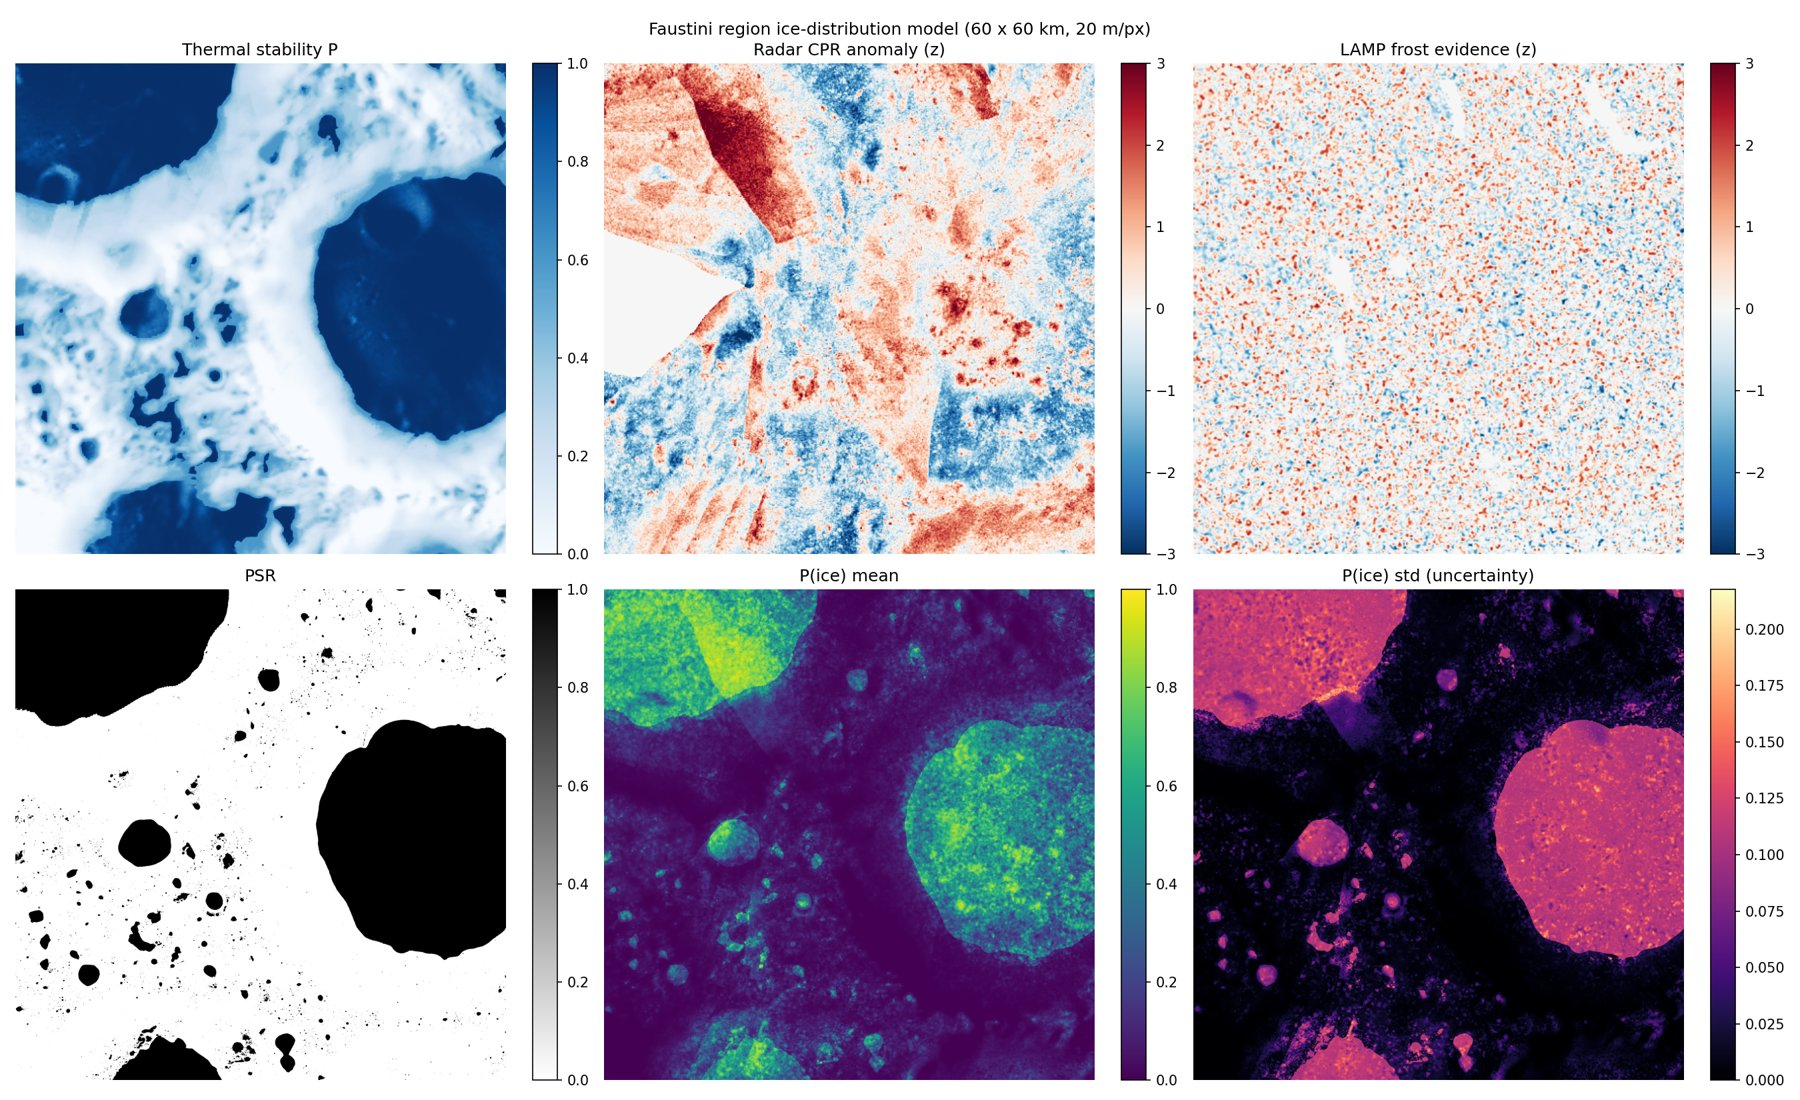
\includegraphics[width=\linewidth]{images/ice_probability.jpg}
\caption{Evidence layers and fused result: thermal stability, roughness-corrected Mini-RF CPR
anomaly, LAMP frost evidence, PSR mask, mean $\Pice$ and its Monte-Carlo standard deviation.}
\end{figure}

\subsection{Dual-frequency inversion}

\begin{center}
\begin{tabularx}{\linewidth}{@{}Xr@{}}
\toprule
Quantity & Value \\
\midrule
Noise $\sigma_L$ / $\sigma_S$ & 0.029 / 0.117 \\
Baseline L ($\rho=-\mathrm{SERD}$) & $a=3.61$, $b=6.32$ \\
Baseline S & $a=0.482$, $b=1.57$ \\
$k=k_L/k_S$ (calibrated on 3484 px) & 0.347 \\
Area: none / L+S / L only / S only & 2260.1 / 3.9 / 44.0 / 81.9\,km$^2$ \\
Enrichment $E_1$ (L+S) & 1.16 \\
Enrichment $E_2$ (L only) & 0.66 \\
Enrichment $E_3$ (S only) & 3.55 \\
Depth signal significant & no \\
Median depth where $\Pice>0.5$ & 1.53\,m \\
\bottomrule
\end{tabularx}
\end{center}

Neither physically meaningful class is enriched in cold terrain by the required factor of two,
so the depth map is shown for inspection but not used in the volume. The ``S only'' class is
enriched by 3.5, which points to a systematic difference between the Mini-RF and DFSAR products
(resolution, incidence angle or calibration) rather than to ice, since an S-only detection
cannot be produced by the attenuation model. A proper DFSAR S-band mosaic should remove this
inconsistency.

\begin{figure}[H]
\centering
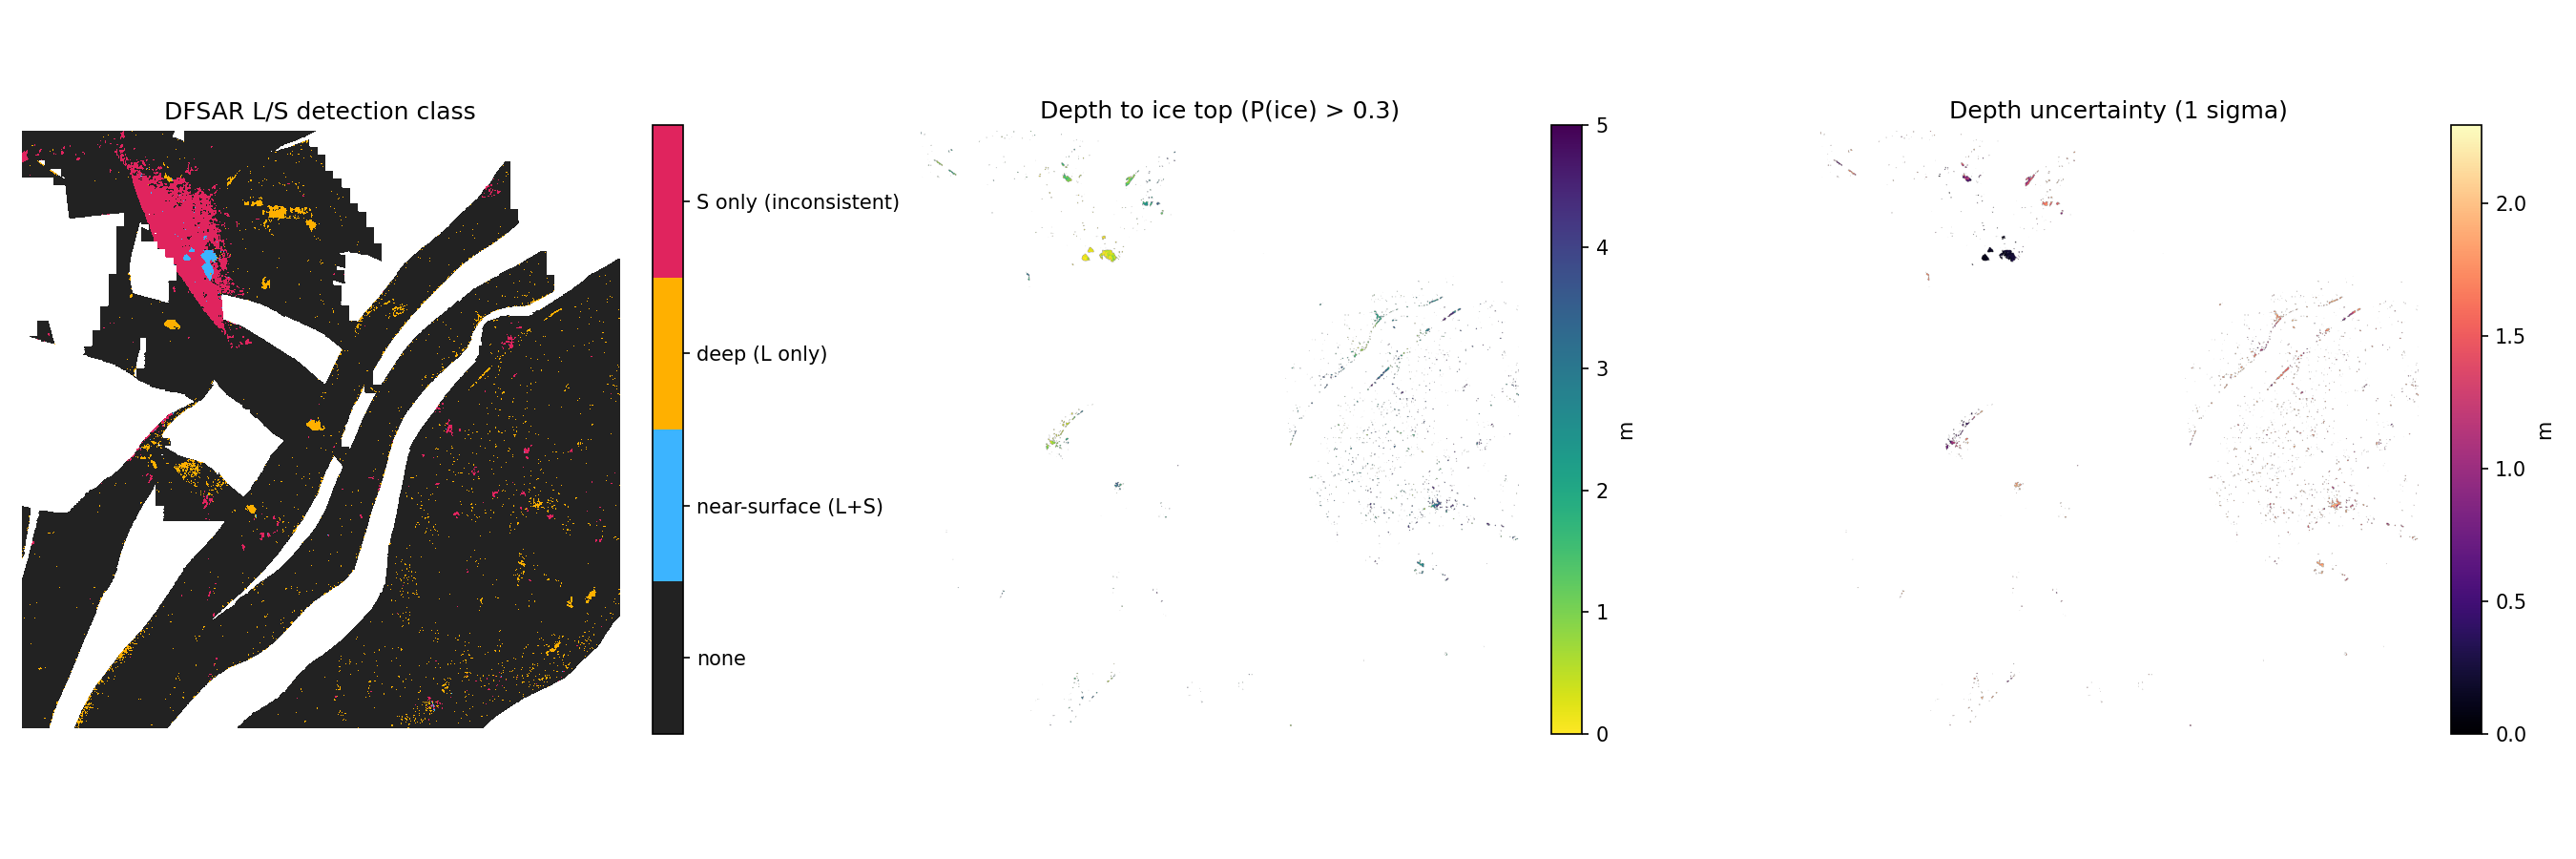
\includegraphics[width=\linewidth]{images/ice_depth.png}
\caption{DFSAR L/S detection class, depth to the top of the ice where $\Pice>0.3$, and its
$1\sigma$ Monte-Carlo uncertainty.}
\end{figure}

\subsection{Traverse}
No planner output is committed (\code{outputs/} is git-ignored), so this report does not quote a
path length or slope statistics. Running \code{python path\_planner.py} reproduces them from the
public DEM.

\subsection{Tests}
\code{tests/test\_dfsar.py} checks the canonical full-pol targets, that unpolarised noise gives
$\mathrm{CPR}\approx1$ and low DOP, that a fully polarised wave gives $\mathrm{DOP}=1$, and that
the dual-band inversion on a synthetic scene (warm ice-free third, cold surface-ice third, cold
buried-ice third with $D$ from 0.2 to 2\,m) recovers $k$, keeps the warm false-positive rate
below 2\,\%, classifies over 95\,\% of surface ice as class~1 with median depth below 0.1\,m,
recovers buried depths within 0.2\,m and reports the deepest ice as L-only deeper than 1\,m. All
four tests pass.

%====================================================================
\section{Limitations}\label{sec:limits}
%====================================================================

\begin{itemize}
  \item \textbf{No ground truth.} Weights are priors with wide uncertainty, not fitted values.
        The standard-deviation map shows how much the answer depends on them.
  \item \textbf{S-band substitute.} The L/S inversion uses Mini-RF instead of DFSAR S-band.
        The enrichment test currently rejects the depth map.
  \item \textbf{Fixed ice fraction.} Volumes scale linearly with the assumed $f_{\mathrm{ice}}$;
        the dielectric inversion is not implemented.
  \item \textbf{Extrapolation.} Below 3\,m the volume is extrapolated beyond the L-band sensing
        depth and is reported separately.
  \item \textbf{Planner scope.} The cost map uses slope only. The weighted multi-term cost
        (roughness, illumination, ice probability, hazards, PSR boundary), the
        \code{constraints.json} limits, battery and charging logic, the PPO agent and the
        rover/relay/orbiter simulation described in the README are not implemented.
  \item \textbf{Landing site.} The landing-site code is a prototype with synthetic illumination
        on a different DEM, and is not coupled to the ice map or the planner.
  \item \textbf{Unused layers.} LOLA illumination and DFSAR T-ratio are fetched but not used;
        OHRC boulder and crater hazards are not ingested.
\end{itemize}

%====================================================================
\section{Outlook}
%====================================================================

The most valuable next step is DFSAR S-band (and DOP) for the same area, which would make the
depth inversion self-consistent and allow the enrichment test to be re-run. The T-ratio layer can
then constrain permittivity and hence $f_{\mathrm{ice}}$. On the planning side, the ice
probability, LOLA illumination and PSR-distance layers already exist on the same grid, so the
weighted cost map is mostly a matter of combining arrays; adding the per-day traverse, battery
range and charging constraints turns A* into a resource-constrained search, and landing-site
selection can then be posed as choosing the start node that minimises path cost to the
high-$\Pice$ target subject to slope and illumination limits.

\end{document}
